\documentclass[conference]{IEEEtran}
\usepackage{cite}
\usepackage{amsmath,amssymb,amsfonts}
\usepackage{graphicx}
\graphicspath{{figures/}}
\usepackage{booktabs}
\usepackage{array}
\usepackage{tabularx}
\usepackage{textcomp}
\usepackage{xcolor}
\usepackage{url}
\begin{document}

\title{Factors Associated with Female Participation in the Job Market}

\author{\IEEEauthorblockN{Suryansh Rohil \quad Anant Atreya}
\IEEEauthorblockA{Roll numbers: 2310110314 and 2310110038\\
Course: DOM207--DOM3007--DOM6401\\
Instructor: Mr. Jaideep Ghosh\\
Client: Government of India}}

\maketitle

\begin{abstract}
Of the 753 records in the supplied workbook, 428 are marked as participating in the workforce. In the prespecified logistic model, one additional child under six is associated with a 17.5 percentage point lower average participation probability. The nonwife income coefficient is negative, though its construction changes with participation status. Probit and linear probability estimates give similar signs. Stratified five fold validation gives an area under the receiver operating characteristic curve of 0.854. The interaction block is not supported, and single record deletion changes both interaction coefficient signs. These estimates describe the supplied records, not causal effects or population averages.
\end{abstract}

\begin{IEEEkeywords}
labor-force participation, logistic regression, family income, nonwife income, marginal effects
\end{IEEEkeywords}

\section{Introduction}
The Government of India assignment asks which observed characteristics are associated with women's participation in the job market. We treat the supplied workbook as client data collected by an appointed third-party agency and do not add records or alter its contents~\cite{task,data}. Its description defines \texttt{inlf} as participation in the workforce in 2019. The analysis therefore estimates associations within these 753 records.

The explanatory framework follows household labor-supply theory: education and experience can change the return to paid work, while young children and resources outside the woman's own earnings can alter the trade between work and household time~\cite{becker,mroz}. The workbook includes age, education, actual experience, children by age, family income, a marginal tax rate, neighborhood unemployment, and city residence. It does not provide a sampling frame, survey weights, or enough design information to establish population representativeness. We make no causal claim.

\section{Data Preprocessing}
The worksheet contains 753 records and 20 columns. The participation indicator is one for 428 records and zero for 325. The observed share is 56.8\%. All 325 zero-participation rows use a period in \texttt{sal}; the 428 participation rows have numeric values. No other model field is missing. The script keeps these salary entries missing in the source copy and substitutes zero only in the earnings product where hours are zero.

We recomputed the required variable for every record:
\[
\texttt{nwifeinc}_i = \frac{\texttt{faminc}_i - \texttt{sal}_i\,\texttt{hours}_i}{1000}.
\]
The supplied workbook already contains \texttt{nwifeinc}. The maximum absolute difference between that column and the recomputed value is $0.000006$, within the $10^{-4}$ comparison tolerance. Values are expressed in thousands of the workbook's income units.

The supporting analysis script and report source are maintained in the project repository~\cite{repo}.

\texttt{nwifeinc} is intended to measure household resources other than the woman's own earnings. Its construction changes with participation status. For nonparticipants, hours are zero and the value is family income divided by 1000. For participants, estimated own earnings are subtracted. The resulting predictor is mechanically linked to the employment decision and is not a clean measure of exogenous nonlabor income. We interpret its coefficient as an adjusted association and compare it with a model that substitutes \texttt{faminc}; the two income measures are never entered together.

The primary and sensitivity roles of the other variables are listed in Table~\ref{tab:variables}.

\begin{table*}[!t]
\centering
\caption{Variable roles in the participation analysis.}
\label{tab:variables}
\small
\begin{tabularx}{\textwidth}{>{\raggedright\arraybackslash}p{0.19\textwidth}>{\raggedright\arraybackslash}p{0.28\textwidth}>{\raggedright\arraybackslash}X}
\toprule
Role & Variables & Reason \\
\midrule
Primary model & \texttt{kidslt6}, \texttt{kidsge6}, age, education, experience, \texttt{nwifeinc}, \texttt{mtr}, \texttt{unem}, \texttt{city} & Household constraints, human capital, nonwife resources, tax incentives, and local conditions. Age and experience enter quadratically. \\
Specified interactions & \texttt{kidslt6}$\times$\texttt{nwifeinc}; education$\times$\texttt{city} & Test whether the child-count association varies with household resources and whether the education association differs by city residence. \\
Sensitivity models & \texttt{faminc}; \texttt{husage}, \texttt{hused}, \texttt{hushrs}; \texttt{momed}, \texttt{daded}; categorical \texttt{kidslt6}; model without \texttt{mtr} & Assess alternative income construction, spouse and family background controls, child-count form, and tax-rate timing. \\
Excluded as direct predictors & \texttt{sal}, \texttt{hours}, \texttt{repsal}, \texttt{hussal} & The woman's salary and hours depend on employment; \texttt{repsal} refers to a 2020 interview after the 2019 outcome period. Husband's wage overlaps with family resources in \texttt{nwifeinc}. \\
\bottomrule
\end{tabularx}
\end{table*}

We did not delete observations. The child variables are nonnegative counts. The workbook gives women's age from 30 to 60 years and actual experience from 0 to 45 years. We centered age, education, experience, and \texttt{nwifeinc} before constructing powers and products. The model's \texttt{mtr} term is ten times the supplied rate, so one unit represents a 10 percentage-point rate increase.

\section{Data Visualization}
The sample has lower participation rates among records with more children under six. The third-child category contains only three observations, so its zero observed rate is not treated as a stable population estimate. Fig.~\ref{fig:participation} shows the outcome counts and the observed rates by child count. Fig.~\ref{fig:profiles} displays age, education, experience, and nonwife income by observed participation status; these are descriptive contrasts.

\begin{figure*}[!t]
\centering
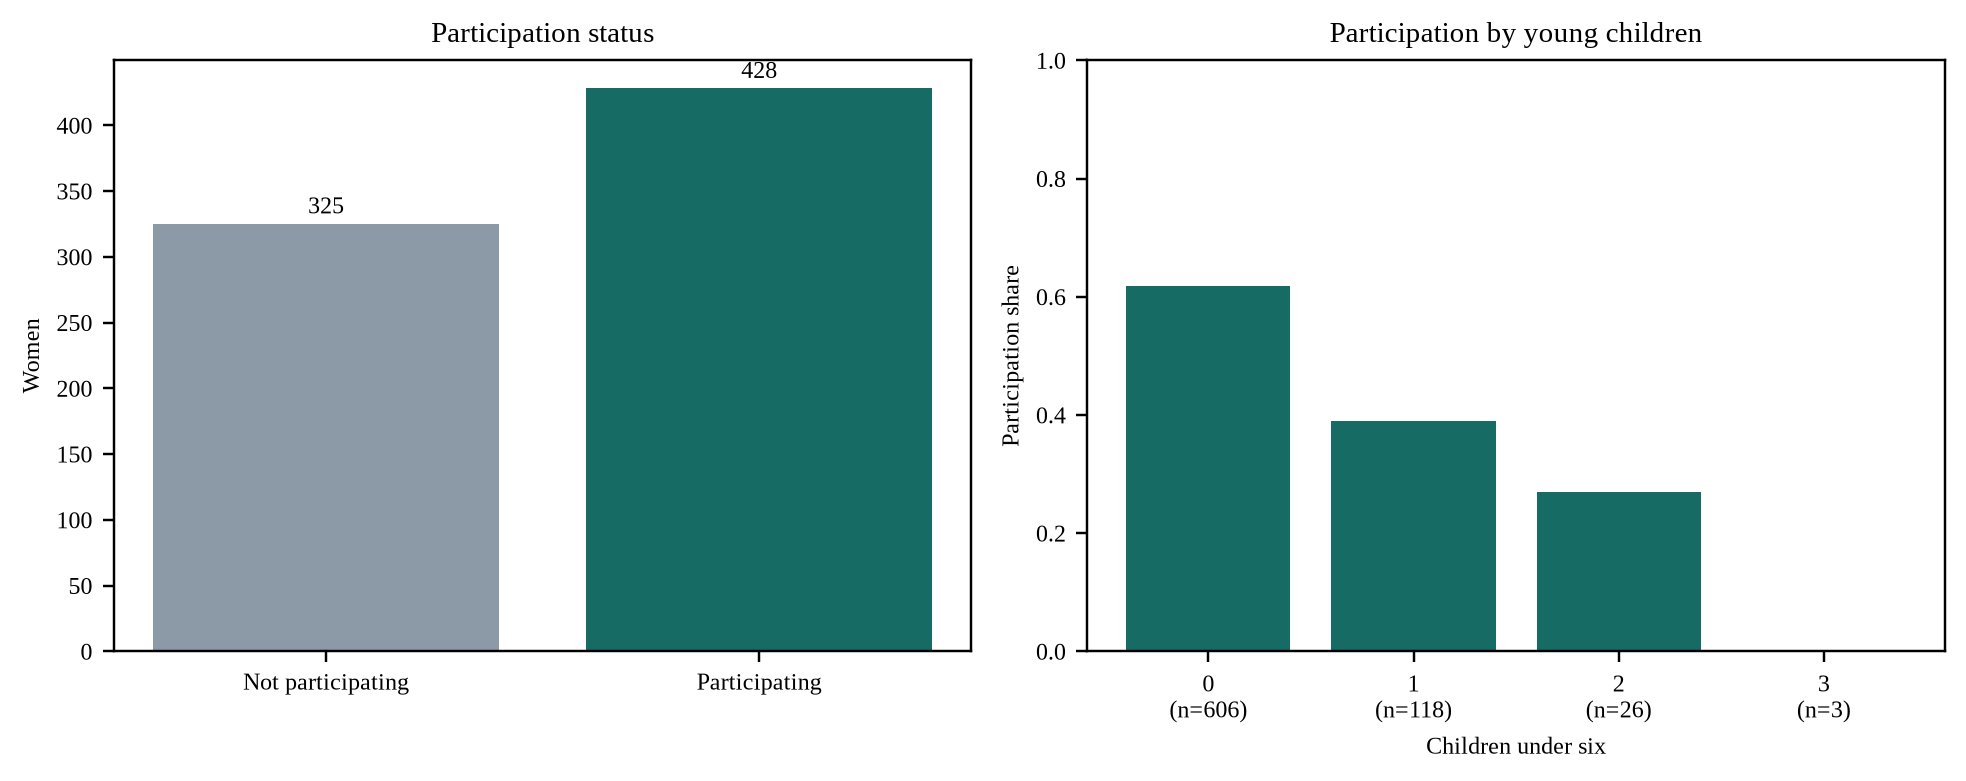
\includegraphics[width=0.95\textwidth]{participation.png}
\caption{Participation counts and observed participation shares by the number of children under six. Sample sizes are shown under each child-count value.}
\label{fig:participation}
\end{figure*}

\begin{figure*}[!t]
\centering
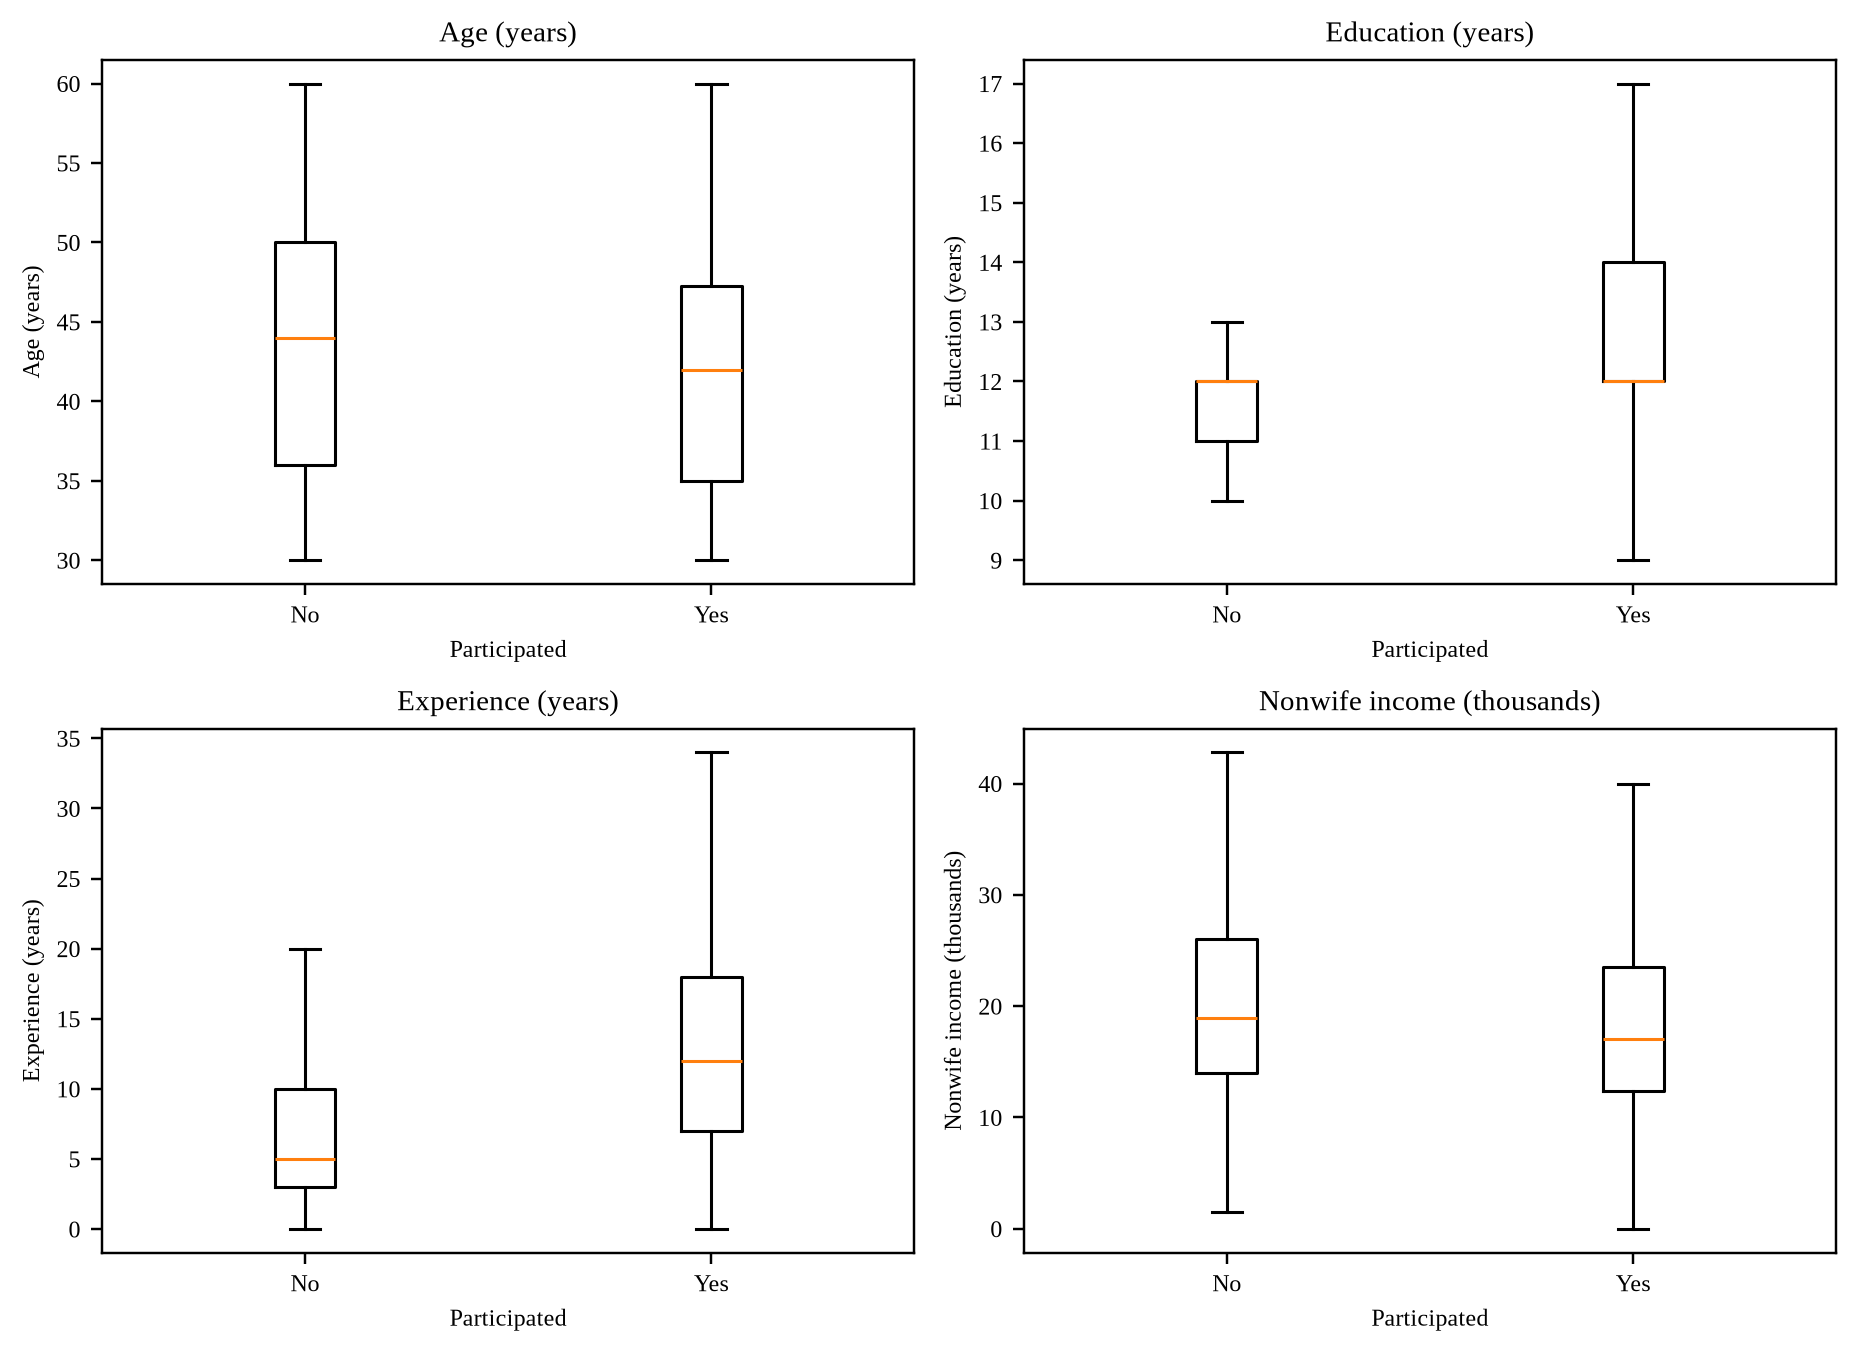
\includegraphics[width=0.88\textwidth]{profiles.png}
\caption{Distributions of selected predictors by observed participation. Nonwife income is mechanically constructed using the woman's estimated earnings.}
\label{fig:profiles}
\end{figure*}

Fig.~\ref{fig:interaction} plots model probabilities at city residence zero, holding the other predictors at their sample means or medians. The horizontal range spans the 5th to 95th percentiles of nonwife income. Fig.~\ref{fig:validation} reports out-of-fold discrimination and calibration. The area under the receiver operating characteristic (ROC) curve, or AUC, summarizes ranking; the reliability curve compares predicted probabilities with observed shares~\cite{fawcett,calibration,sklearn}. The in-sample ROC curve is included only to show its difference from cross-validated performance.

\begin{figure}[!t]
\centering
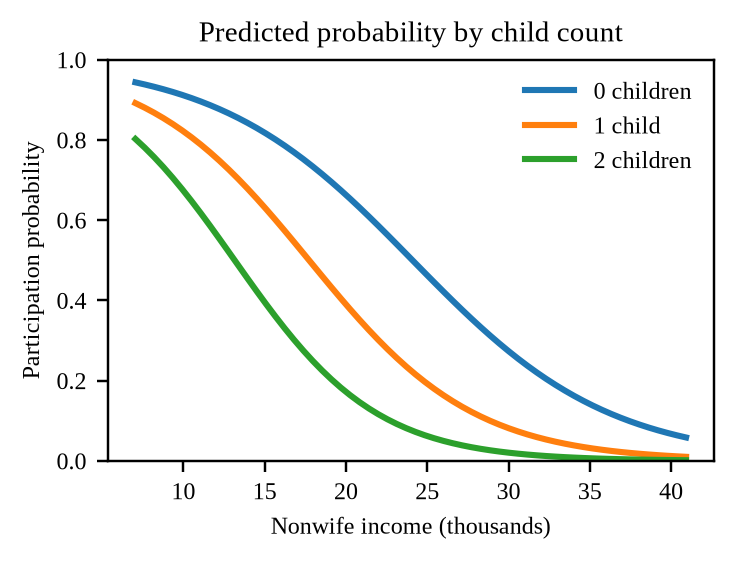
\includegraphics[width=0.95\columnwidth]{interaction.png}
\caption{Predicted participation probability over nonwife income for zero, one, and two children under six, with city residence fixed at zero.}
\label{fig:interaction}
\end{figure}

\begin{figure*}[!t]
\centering
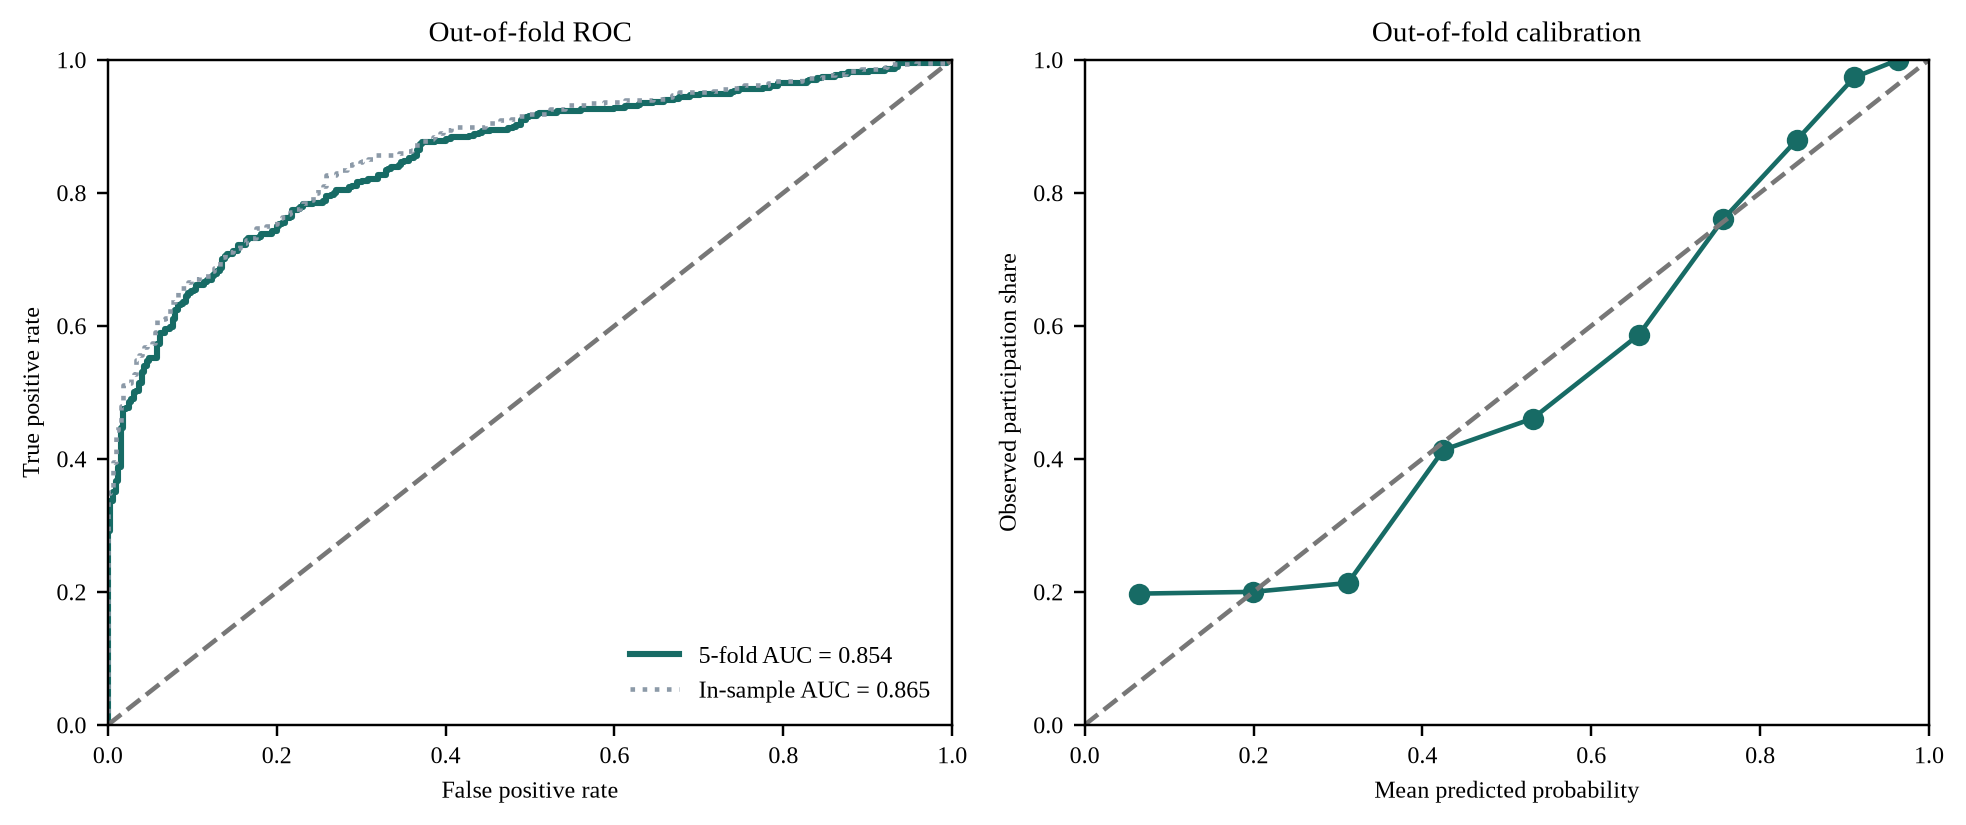
\includegraphics[width=0.92\textwidth]{roc_calibration.png}
\caption{In-sample and five-fold out-of-fold ROC curves, with the out-of-fold calibration curve.}
\label{fig:validation}
\end{figure*}

\section{Hypotheses or Theory Building}
Household time-allocation theory predicts that additional resources outside the woman's own earnings can reduce the need to supply labor when leisure is a normal good~\cite{becker}. Prior labor-supply analysis also shows why estimated relationships depend on the model's economic and statistical assumptions~\cite{mroz}. Before estimating the outcome models, we fixed these directional hypotheses:

\begin{enumerate}
\item Each additional child under six is associated with lower participation. A positive interaction with nonwife income is expected if household resources ease the care-cost constraint.
\item Higher nonwife income is associated with lower participation through an income effect. Its construction in this workbook prevents a causal interpretation.
\item Education and experience are associated with higher participation. The experience association may be concave as accumulated human capital rises at a decreasing rate.
\item The education association may be stronger in a city, where access to paid work and the mix of jobs can differ.
\item Age has a nonlinear association with participation over the observed age range as family responsibilities and retirement proximity change.
\end{enumerate}

These directions determined the model terms before estimation. We report unsupported and contrary results as well as supported ones. No interaction was retained or dropped on the basis of its individual p-value.

\section{Analysis}
\subsection{Specification and fit}
We estimated logit and probit by maximum likelihood~\cite{statsmodels}. The primary logit specification has 13 slope terms and an intercept. It includes the two child counts, centered age and age squared, centered education, centered experience and experience squared, centered \texttt{nwifeinc}, \texttt{mtr}, neighborhood unemployment, city residence, and the two prespecified interactions. The \texttt{mtr} regressor is scaled so a one-unit change represents a 10 percentage-point increase. The sample supplies 428 participation cases and 325 nonparticipation cases, or 32.9 and 25.0 cases per slope term, respectively.

\begin{IEEEeqnarray}{rCl}
\Pr(\texttt{inlf}_i=1\mid X_i) &=& \Lambda(\eta_i),\\
\eta_i &=& \beta_0 + \beta_1\texttt{kidslt6}_i \nonumber\\
& & + \beta_2\texttt{kidsge6}_i + \beta_3\texttt{age\_c}_i \nonumber\\
& & + \beta_4\texttt{age\_sq}_i + \beta_5\texttt{ed\_c}_i \nonumber\\
& & + \beta_6\texttt{exper\_c}_i + \beta_7\texttt{exper\_sq}_i \nonumber\\
& & + \beta_8\texttt{nwifeinc\_c}_i + \beta_9(10\texttt{mtr}_i) \nonumber\\
& & + \beta_{10}\texttt{unem}_i + \beta_{11}\texttt{city}_i \nonumber\\
& & + \beta_{12}(\texttt{kidslt6}_i \times \texttt{nwifeinc\_c}_i) \nonumber\\
& & + \beta_{13}(\texttt{ed\_c}_i \times \texttt{city}_i).
\end{IEEEeqnarray}
Here, $\Lambda$ is the logistic cumulative distribution function.

Table~\ref{tab:logit} reports the full coefficient estimates. The quadratic block improves fit relative to the linear main-effects model, $\chi^2(2)=10.80$, $p=0.0045$. The interaction block does not, $\chi^2(2)=2.46$, $p=0.292$. Within the full model, experience squared is negative ($\hat\beta=-0.0032$, $p=0.0057$); age squared is not distinguishable from zero ($p=0.355$). McFadden's pseudo-$R^2$ is 0.300. The in-sample AUC is 0.865 and Brier score is 0.151. Stratified five-fold cross-validation gives pooled out-of-fold AUC 0.854, with fold values from 0.834 to 0.867.

\begin{table*}[!t]
\centering
\caption{Full logit coefficient estimates. Standard errors are conventional maximum-likelihood estimates.}
\label{tab:logit}
\small
\begin{tabular}{lrrr}
\toprule
Term & Estimate & Std. error & $p$-value \\
\midrule
Children under six & $-1.128$ & 0.224 & $<0.001$ \\
Children aged 6--18 & 0.261 & 0.085 & 0.002 \\
Age, centered & $-0.064$ & 0.016 & $<0.001$ \\
Age squared & $-0.0015$ & 0.0016 & 0.355 \\
Education, centered & 0.127 & 0.076 & 0.093 \\
Experience, centered & 0.121 & 0.016 & $<0.001$ \\
Experience squared & $-0.0032$ & 0.0012 & 0.006 \\
Nonwife income, per 1,000 units, centered & $-0.165$ & 0.023 & $<0.001$ \\
Marginal tax rate, per 10 percentage points & $-2.351$ & 0.307 & $<0.001$ \\
Neighborhood unemployment & $-0.030$ & 0.030 & 0.325 \\
City residence & $-0.101$ & 0.207 & 0.625 \\
Children under six $\times$ nonwife income & $-0.032$ & 0.022 & 0.138 \\
Education $\times$ city & 0.016 & 0.092 & 0.866 \\
\bottomrule
\end{tabular}
\end{table*}

\subsection{Probability-scale effects}
The logit estimates are easier to compare with the sample when expressed as average marginal effects (AMEs). The child count is treated as linear, so its AME is the average derivative for one additional child. City residence is reported as a discrete change from zero to one. Confidence intervals use the delta method. Table~\ref{tab:ame} reports the probability-scale estimates.

\begin{table*}[!t]
\centering
\caption{Logit average marginal effects on participation probability. Values are percentage points.}
\label{tab:ame}
\small
\begin{tabular}{lrrr}
\toprule
Variable and unit & AME & 95\% lower & 95\% upper \\
\midrule
One additional child under six & $-17.5$ & $-24.0$ & $-11.1$ \\
One additional child aged 6--18 & 4.1 & 1.5 & 6.7 \\
One year of age & $-1.0$ & $-1.5$ & $-0.5$ \\
One year of education & 2.2 & 0.7 & 3.6 \\
One year of experience & 2.0 & 1.6 & 2.4 \\
Nonwife income, per 1,000 units & $-2.7$ & $-3.4$ & $-2.1$ \\
Marginal tax rate, per 10 percentage points & $-37.1$ & $-45.4$ & $-28.9$ \\
One-point increase in neighborhood unemployment & $-0.5$ & $-1.4$ & 0.5 \\
City versus noncity residence & $-1.6$ & $-8.0$ & 4.7 \\
\bottomrule
\end{tabular}
\end{table*}

The estimated child-count association becomes more negative over the observed nonwife income quartiles: $-11.5$ percentage points at $13.0$ thousand, $-14.7$ at $17.7$ thousand, and $-17.4$ at $24.5$ thousand. The interaction coefficient has the opposite sign to the prespecified expectation and is not significant. The joint test also fails to support the interaction block. These conditional estimates are not evidence that income increases the cost of child care.

\subsection{Sensitivity specifications}
The sign of the child-count estimate is negative across each reported specification. The income coefficient is sensitive to its definition and to inclusion of \texttt{mtr}. Table~\ref{tab:sensitivity} reports selected logit coefficients; income is in thousands of workbook units. McFadden's pseudo-$R^2$ is shown as a fit description, not as a causal criterion.

\begin{table*}[!t]
\centering
\caption{Selected sensitivity estimates.}
\label{tab:sensitivity}
\small
\begin{tabularx}{\textwidth}{Xrrrr}
\toprule
Specification & Child term & Income term & Child-income term & Pseudo-$R^2$ \\
\midrule
Primary logit & $-1.128$ & $-0.165$ & $-0.032$ & 0.300 \\
Without \texttt{mtr} & $-1.428$ & $-0.021$ & $-0.005$ & 0.222 \\
Substitute \texttt{faminc} & $-1.374$ & $-0.001$ & $-0.014$ & 0.222 \\
Add husband age, education, and hours & $-1.148$ & $-0.160$ & $-0.031$ & 0.308 \\
Add parental education & $-1.125$ & $-0.165$ & $-0.032$ & 0.300 \\
Categorical child count & $-1.137$ for one child & $-0.167$ & $-0.020$ for one child & 0.300 \\
\bottomrule
\end{tabularx}
\end{table*}

The \texttt{faminc} coefficient is $-0.0011$ with $p=0.947$; this measure includes the woman's earnings for participants and is not equivalent to \texttt{nwifeinc}. Removing \texttt{mtr} changes the nonwife income coefficient from $-0.165$ to $-0.021$ and lowers pseudo-$R^2$ from 0.300 to 0.222. The primary-model correlation between \texttt{mtr} and \texttt{nwifeinc} is $-0.810$. The two VIF values are 3.95 and 3.98. Husband education is negative in its sensitivity model ($p=0.032$); husband age is not significant, and husband hours is marginal at $p=0.060$. Parental education terms are not significant. These estimates depend on the specified controls and do not isolate causal effects.

\subsection{Assumptions and limits}
The model assumes that the listed predictors adequately describe the conditional participation probability and that records are independent. Independence cannot be tested from this workbook because household identifiers and sample-design details are absent. Logit does not require a constant conditional error variance. For a binary outcome, the conditional variance is $p(1-p)$. The linear-probability model therefore uses HC3 heteroskedasticity-consistent standard errors; 7.8\% of its fitted values fall outside $[0,1]$.

The largest variance inflation factor (VIF) values are 3.98 for \texttt{nwifeinc} and 3.95 for \texttt{mtr}. Their correlation is $-0.810$. Removing \texttt{mtr} changes the income estimate, so the two coefficients should not be read as independent mechanisms. The \texttt{mtr} definition refers to a woman on payroll and may be partly determined after participation. Its negative estimate is not used as a basis for a policy recommendation.

In the spouse-control model, VIF is 1.11 for husband hours, 5.02 for husband age, and 4.00 for \texttt{nwifeinc}. Adding husband's hourly wage for a collinearity check raises the \texttt{nwifeinc} VIF to 5.16; the \texttt{hussal} VIF is 4.18, and its pairwise correlation with \texttt{nwifeinc} is 0.758. This supports leaving husband's wage out of the primary model. Husband hours remain in the named sensitivity model, where their VIF is low.

The logit fit converged. The cross-tabulation of child count by city shows only three records with three children under six, and none has \texttt{inlf}=1. This cell pattern warns against treating the third-child rate as stable and raises separation concerns for categorical specifications. We use a linear count in the primary model. The categorical sensitivity combines counts of two or more; its negative coefficients are not evidence about the separate third-child effect. The combined category has a coefficient of $-2.683$ ($p=0.002$), but it cannot identify a separate effect for three children.

Influence checks identify workbook row 120 as the largest Cook-distance case ($D=0.210$); 42 records exceed the descriptive $4/n$ screening value. Row 403 has the largest absolute deviance residual (4.34). All 753 leave-one-record refits converged. Deleting row 120 changes the \texttt{kidslt6}$\times$\texttt{nwifeinc} coefficient by 0.0346 from its full-sample value of $-0.0321$. Deleting row 403 changes the education by city coefficient by 0.0256 from 0.0156. Either coefficient can change sign after one deletion. Their joint test is not significant. The primary average marginal effects change less: at most 0.83 percentage points for the child count and 0.35 points per 1,000 income units. We do not interpret either interaction as a policy effect.

Five-fold AUC summarizes discrimination within this sample, not performance on a new survey. No sampling frame, response rate, weights, regional identifiers, or contemporaneous external measures are supplied. The report retains the assignment's Government of India client framing, while limiting conclusions to associations in the observed workbook. The analysis cannot establish causal effects or national population averages.

\section{Recommendations}
\begin{enumerate}
\item \textbf{Evaluate access to care for young children.} Each additional child under six is associated with a 17.5 percentage point lower average participation probability (95 percent confidence interval: $-24.0$ to $-11.1$). The negative sign remains in the family-income and spouse-control specifications. This supports evaluating childcare access as a possible constraint, not claiming that a childcare program will increase participation. The three records with three young children are too few for a separate estimate.
\item \textbf{Test experience recognition and return-to-work training.} The experience AME is 2.0 percentage points per year, while the squared experience coefficient is negative and significant ($p=0.006$). This pattern is consistent with a diminishing association in this sample. A return-to-work program should be evaluated against a comparison group before any effect is attributed to training.
\item \textbf{Do not target interventions by city status from these estimates.} The city AME is $-1.6$ percentage points, with a 95\% interval from $-8.0$ to 4.7. The education by city interaction has $p=0.866$ and changes sign under deletion of one record. The sample supplies no support for different city-based education policy.
\item \textbf{Clarify income and tax measures before interpreting incentives.} The required \texttt{nwifeinc} estimate is negative, but its calculation differs between participants and nonparticipants. The alternative \texttt{faminc} coefficient is near zero and includes the woman's earnings. The $-0.810$ correlation between \texttt{mtr} and \texttt{nwifeinc}, and the change after removing \texttt{mtr}, make a data-definition review necessary before using either estimate to assess household income or tax policy.
\item \textbf{Establish the sample design before extending these findings.} Obtain the sampling frame, weights, response process, and geographic identifiers, then repeat the prespecified model on a documented sample. The current workbook supports associations for these records only.
\end{enumerate}

\begin{thebibliography}{00}
\bibitem{task} DOM207--DOM3007--DOM6401, ``MP4: Women's Participation in the Job Market,'' supplied project specification, 2026.
\bibitem{data} \textit{IWomenJob.xlsx}, supplied workbook, sheets ``IWomenJob'' and ``Description,'' 2026.
\bibitem{becker} G. S. Becker, ``A theory of the allocation of time,'' \textit{The Economic Journal}, vol. 75, no. 299, pp. 493--517, 1965. doi: 10.2307/2228949.
\bibitem{mroz} T. A. Mroz, ``The sensitivity of an empirical model of married women's hours of work to economic and statistical assumptions,'' \textit{Econometrica}, vol. 55, no. 4, pp. 765--799, 1987. doi: 10.2307/1911029.
\bibitem{repo} S. Rohil and A. Atreya, ``DOM207 MP4 participation analysis,'' GitHub repository. Available at \url{https://github.com/s-uryansh/DOM207/tree/main/MP4}. Accessed: Nov. 9, 2026.
\bibitem{fawcett} T. Fawcett, ``An introduction to ROC analysis,'' \textit{Pattern Recognition Letters}, vol. 27, no. 8, pp. 861--874, 2006. doi: 10.1016/j.patrec.2005.10.010.
\bibitem{calibration} A. Niculescu-Mizil and R. Caruana, ``Predicting good probabilities with supervised learning,'' in \textit{Proceedings of the 22nd International Conference on Machine Learning}, pp. 625--632, 2005. doi: 10.1145/1102351.1102430.
\bibitem{sklearn} Scikit-learn developers, ``StratifiedKFold, roc\_auc\_score, and calibration\_curve,'' API documentation. Available at \url{https://scikit-learn.org/stable/}.
\bibitem{statsmodels} S. Seabold and J. Perktold, ``Statsmodels: econometric and statistical modeling with Python,'' in \textit{Proceedings of the 9th Python in Science Conference}, pp. 92--96, 2010. Documentation: \url{https://www.statsmodels.org/dev/generated/statsmodels.discrete.discrete_model.Logit.html}.
\end{thebibliography}
\end{document}
